\documentclass{beamer}

\usepackage{tikz}
\usepackage{booktabs} % Tables: \toprule, \midrule, \bottomrule

\usetheme{Madrid}
\usecolortheme{default}

% =========================
% Title information
% =========================

\title[Short Title]{Presentation Title}

\subtitle{Presentation Subtitle}

\author[Lyu Shenghao]{
    Lyu Shenghao\inst{1,2}
}

\institute[Tsinghua \& CIAE]{
    \inst{1}
    Tsinghua University, Beijing, China
    \and
    \inst{2}
    China Institute of Atomic Energy, Beijing, China
}

\date{\today}


% =========================
% Watermark
% =========================

\newcommand{\mywatermark}{
    \begin{tikzpicture}[remember picture,overlay]
        \node[
            opacity=0.1,
            xshift=2cm,
            yshift=-0.4cm,
            at=(current page.center)
        ] {
            \includegraphics[
                width=0.52\paperwidth
            ]{logo_background.png}
        };
    \end{tikzpicture}
}

% Draw the watermark on every page except the title page.
\setbeamertemplate{background}{%
    \ifnum\value{page}>1\relax
        \mywatermark
    \fi
}



% =========================
% Color and font settings
% =========================

% Use native Beamer / Madrid colors and fonts.
% No custom color or font definitions are applied.


% =========================
% Document
% =========================

\begin{document}

% =========================
% Title page
% No watermark
% Logos remain in original position
% =========================

{


\begin{frame}

    \titlepage

    \begin{tikzpicture}[remember picture,overlay]
        \node[
            anchor=south,
            yshift=1cm
        ] at (current page.south) {

            \makebox[0.4\paperwidth]{
                \raisebox{0.07cm}{
                    \includegraphics[height=0.72cm]{logo_tsinghua}
                }
                \hfill
                \includegraphics[height=0.8cm]{logo_cnnc}
            }

        };
    \end{tikzpicture}

\end{frame}
}


% =========================
% Table of contents
% Watermark is automatically restored
% =========================

\begin{frame}
    \frametitle{Table of Contents}
    \tableofcontents
\end{frame}

% =========================
% Basic syntax examples
% Copy or remove frames as needed.
% =========================

\section{Text and Layout}

\begin{frame}{Text and Lists}
    \textbf{Bold}, \textit{italic}, \underline{underlined},
    and \alert{highlighted} text.

    \medskip % Spacing: \smallskip, \medskip, \bigskip

    \begin{itemize}
        \item First point
        \item Second point
        \begin{itemize}
            \item Nested point
        \end{itemize}
    \end{itemize}

    \begin{enumerate}
        \item First step
        \item Second step
    \end{enumerate}

    {\footnotesize A smaller note.}
    \hfill\href{https://example.com}{Link text}
\end{frame}

\begin{frame}[t]{Terms and Notes}
    \framesubtitle{Definitions, footnotes, and citations}

    \begin{description}
        \item[Input] Data supplied to a model.
        \item[Output] A prediction returned by the model.
    \end{description}

    A short statement with a source\footnote{Use footnotes for brief notes.}
    and a bibliography citation~\cite{key}.

    \medskip
    Equation~\eqref{eq:linear-system} is defined in the mathematics section.
\end{frame}

\begin{frame}{Blocks}
    \begin{block}{Remark}
        General information.
    \end{block}

    \begin{alertblock}{Important}
        A point that needs attention.
    \end{alertblock}

    \begin{exampleblock}{Example}
        A concrete example.
    \end{exampleblock}
\end{frame}

\begin{frame}{Columns and Images}
    \begin{columns}[T,onlytextwidth]
        \begin{column}{0.48\textwidth}
            \textbf{Left column}
            \begin{itemize}
                \item Explain the figure here.
                \item Use \texttt{\string\textwidth} for local width.
            \end{itemize}
        \end{column}
        \begin{column}{0.48\textwidth}
            \centering
            % Replace with your image file.
            \includegraphics[width=0.65\textwidth]{logo_tsinghua.png}

            \smallskip
            {\footnotesize Figure caption.}
        \end{column}
    \end{columns}
\end{frame}

\section{Mathematics and Graphics}

\begin{frame}{Equations}
    Inline math: $E = mc^2$.

    % Unnumbered display equation
    \[
        f(x) = \frac{1}{\sqrt{2\pi\sigma^2}}
        \exp\left(-\frac{(x-\mu)^2}{2\sigma^2}\right)
    \]

    % Aligned, numbered equations; use align* to omit numbers.
    \begin{align}
        y &= ax + b, \\ 
        \mathbf{A}\mathbf{x} &= \mathbf{b}.
    \end{align}
\end{frame}

\begin{frame}{Matrices and Piecewise Functions}
    % Label numbered equations; reference them with \eqref{...}.
    \begin{equation}
        \begin{pmatrix}
            a & b \\
            c & d
        \end{pmatrix}
        \begin{pmatrix} x_1 \\ x_2 \end{pmatrix}
        = \begin{pmatrix} y_1 \\ y_2 \end{pmatrix}
        \label{eq:linear-system}
    \end{equation}

    \[
        f(x) =
        \begin{cases}
            x^2, & x \geq 0, \\
            -x,  & x < 0.
        \end{cases}
    \]
\end{frame}

\begin{frame}{Tables}
    \centering
    \begin{tabular}{lcc}
        \toprule
        Method & Value & Uncertainty \\
        \midrule
        A & 1.23 & 0.04 \\
        B & 2.34 & 0.05 \\
        \bottomrule
    \end{tabular}
\end{frame}

\begin{frame}{Figures and Cross-References}
    \begin{figure}
        \centering
        % Replace this example image with your own file.
        \includegraphics[height=0.35\textheight]{logo_cnnc.png}
        \caption{Example figure caption.}
        % Place the label after the caption.
        \label{fig:example}
    \end{figure}

    Figure~\ref{fig:example} illustrates a labeled image.
    % For numbered captions, enable:
    % \setbeamertemplate{caption}[numbered]
\end{frame}

\begin{frame}{Simple Workflow}
    \centering
    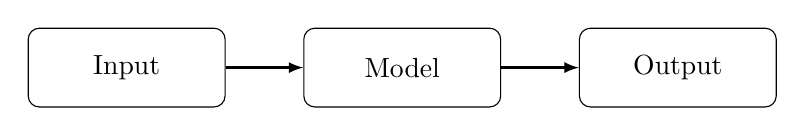
\begin{tikzpicture}[
        workflowbox/.style={draw, rounded corners, align=center,
                     minimum width=2.5cm, minimum height=1cm},
        >=latex
    ]
        \node[workflowbox] (input) at (0,0) {Input};
        \node[workflowbox] (model) at (3.5,0) {Model};
        \node[workflowbox] (output) at (7,0) {Output};
        \draw[->, thick] (input) -- (model);
        \draw[->, thick] (model) -- (output);
    \end{tikzpicture}
\end{frame}

\section{Presentation Techniques}

\begin{frame}{Progressive Reveal}
    % <n-> shows an item from overlay n onward.
    \begin{itemize}
        \item<1-> First point
        \item<2-> Second point
        \item<3-> Third point
    \end{itemize}

    % Alternatives: \pause, \only<2>{...}, \uncover<2->{...}.
\end{frame}

% Code requires a fragile frame. Keep \end{frame} on its own line.
\begin{frame}[fragile]{Code}
\begin{verbatim}
for i in range(3):
    print(i)
\end{verbatim}
\end{frame}

% =========================
% References
% =========================

% Cite an entry with \cite{key} in the main text.
% Add allowframebreaks to the frame options for a long bibliography.
\begin{frame}{References}
    \footnotesize
    \setbeamertemplate{bibliography item}[text]
    \begin{thebibliography}{9}
        \bibitem{key}
        Author, \textit{Title}, Journal (Year).
    \end{thebibliography}
\end{frame}

% =========================
% Optional backup slides
% =========================

% Keep backup slides after the references; remove this example if unused.
\appendix
\section{Appendix}

\begin{frame}{Appendix}
    \begin{itemize}
        \item Supporting calculations or extra results for questions.
        \item Keep the main presentation focused on the key findings.
    \end{itemize}
\end{frame}

\end{document}
